\begin{frame}{Proposed Architecture}
	\small
	\begin{columns}
		\begin{column}{0.6\textwidth}
			The proposed system processes EEG data through cleaning, normalization, and encoding before feeding it into neural models. It supports Dense, RNN, LSTM, and Bi-LSTM architectures with dropout layers for regularization. The models classify sleep stages (W, N1, N2, N3, REM) based on processed input features.
		\end{column}
		\begin{column}{0.3\textwidth}
			\centering
			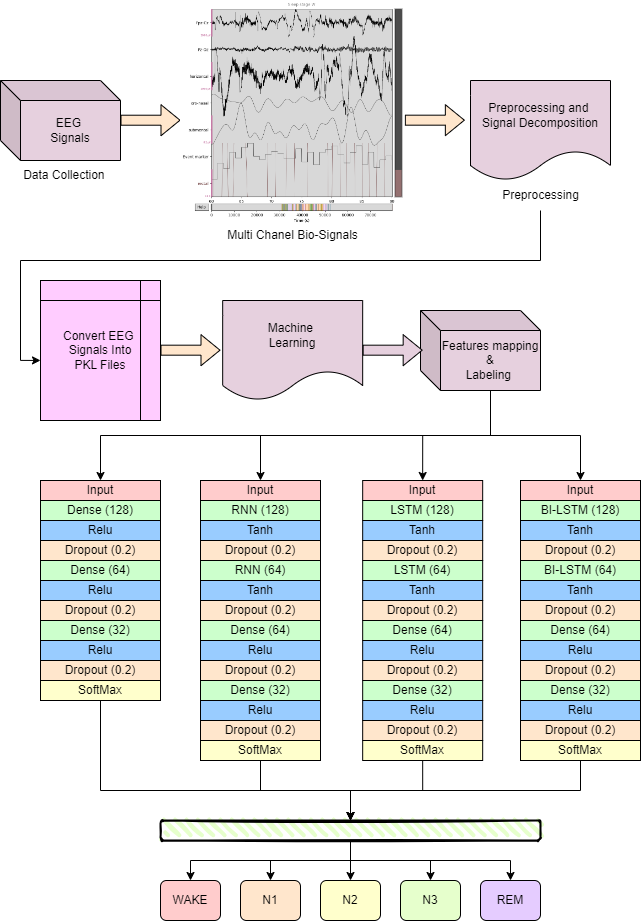
\includegraphics[width=\linewidth]{images/paper_2/aRCHITECHTURE 2} \\
			\textbf{Figure:} Proposed System Architecture
		\end{column}
	\end{columns}
\end{frame}



\begin{frame}{Methodology: Overview and Data Samples}
		\centering
	\small
	\textbf{Proposed System Architecture:} \\[5pt]

	\begin{tabular}{|c|p{0.63\textwidth}|}
		\hline
		\textbf{Component} & \textbf{Description} \\
		\hline
		Input & Sleep EEG Data (.pkl format) \\
		\hline
		Preprocessing & Normalization, Label Encoding, One-hot Encoding, Reshaping \\
		\hline
		Model & Neural Network (Dense / RNN / LSTM / Bi-LSTM) \\
		\hline
		Output & Predicted Sleep Stage (W, N1, N2, N3, REM) \\
		\hline
	\end{tabular} \\[10pt]
	
	\textbf{Sample Input Features and Labels:} \\[5pt]
	\centering
	\begin{tabular}{|p{0.63\textwidth}|c|}
		\hline
		\textbf{Input Features (x)} & \textbf{Label (y)} \\
		\hline
		{[0.059, 0.596, -0.193, ..., -0.601, 0.201]} & W \\
		\hline
		{[-0.022, -0.107, -0.135, ..., 0.038, 0.103]} & W \\
		\hline
		{[... (more samples)]} & N1 \\
		\hline
	\end{tabular} \\[5pt]
	
 
	
\end{frame}



\begin{frame}{Methodology: Label Mapping and Cleaning}
	
	\small
	\textbf{Label Mapping Scheme:} \\[5pt]
	\centering
	\begin{tabular}{|c|c|c|}
		\hline
		\textbf{Original Label} & \textbf{Mapped Label} & \textbf{Meaning} \\
		\hline
		1 & N1 & Light Sleep \\
		\hline
		2 & N2 & Intermediate Sleep \\
		\hline
		3, 4 & N3 & Deep Sleep \\
		\hline
		W & Wake & Awake \\
		\hline
		R & REM & Rapid Eye Movement \\
		\hline
		e & Removed & Unused class \\
		\hline
	\end{tabular} \\[8pt]
	
	
	
	
	\begin{itemize}
		\item Removed invalid entries (e.g., label 'e') using masking.
		\item Encoded valid labels into integers with \texttt{LabelEncoder}.
	\end{itemize}
	
	
	
\end{frame}
 
 






\begin{frame}{Preprocessing Workflow}
	\textbf{Steps involved in data preparation:} \\[10pt]
	\begin{itemize}
		\item \textbf{Loading Data:} Sleep stage data is loaded from `.pkl` files in preprocessed directories.
		\item \textbf{Handling Test Sets:} Ensured test data availability by splitting the training set if necessary.
		\item \textbf{Normalization:} Standardized input features to have zero mean and unit variance.
		\item \textbf{Label Encoding:} Converted sleep stage labels into numerical format.
		\item \textbf{One-Hot Encoding:} Transformed numerical labels into one-hot vectors.
		\item \textbf{Reshaping:} Adjusted input dimensions for model compatibility.
	\end{itemize}
\end{frame}


 

 
 


\begin{frame}{Simple Neural Network Architecture}
	\centering
	\small
	\begin{tabular}{|c|c|c|}
		\hline
		\textbf{Layer Type} & \textbf{Neurons/Units} & \textbf{Activation Function} \\
		\hline
		Input Layer & X\_train & - \\
		\hline
		Dense Layer & 128 & ReLU \\
		\hline
		Dropout Layer & - & 0.2 \\
		\hline
		Dense Layer & 64 & ReLU \\
		\hline
		Dropout Layer & - & 0.2 \\
		\hline
		Dense Layer & 32 & ReLU \\
		\hline
		Dropout Layer & - & 0.2 \\
		\hline
		Output Layer & Number of Classes & Softmax \\
		\hline
	\end{tabular}
	
	\vspace{1em}
	\textit{Model:  Fully Dense Connected Neural Network}
\end{frame}


\begin{frame}{Simple RNN Architecture}
	\centering
	\small
	\begin{tabular}{|c|c|c|}
		\hline
		\textbf{Layer Type} & \textbf{Neurons/Units} & \textbf{Activation Function} \\
		\hline
		Input Layer & X\_train & - \\
		\hline
		RNN Layer 1 & 128 & Tanh \\
		\hline
		Dropout Layer & - & 0.2 \\
		\hline
		RNN Layer 2 & 64 & Tanh \\
		\hline
		Dropout Layer & - & 0.2 \\
		\hline
		Dense Layer & 64 & ReLU \\
		\hline
		Dropout Layer & - & 0.2 \\
		\hline
		Dense Layer & 32 & ReLU \\
		\hline
		Dropout Layer & - & 0.2 \\
		\hline
		Output Layer & Number of Classes & Softmax \\
		\hline
	\end{tabular}
	
	\vspace{1em}
	\textit{Model:  Recurrent Neural Network}
\end{frame}


\begin{frame}{LSTM Architecture}
	\centering
	\small
	\begin{tabular}{|c|c|c|}
		\hline
		\textbf{Layer Type} & \textbf{Neurons/Units} & \textbf{Activation Function} \\
		\hline
		Input Layer & X\_train & - \\
		\hline
		LSTM Layer 1 & 128 & Tanh \\
		\hline
		Dropout Layer & - & 0.2 \\
		\hline
		LSTM Layer 2 & 64 & Tanh \\
		\hline
		Dropout Layer & - & 0.2 \\
		\hline
		Dense Layer & 64 & ReLU \\
		\hline
		Dropout Layer & - & 0.2 \\
		\hline
		Dense Layer & 32 & ReLU \\
		\hline
		Dropout Layer & - & 0.2 \\
		\hline
		Output Layer & Number of Classes & Softmax \\
		\hline
	\end{tabular}
	
	\vspace{1em}
	\textit{Model: Long Short-Term Memory Network}
\end{frame}


\begin{frame}{Bidirectional LSTM Architecture}
	\centering
	\small
	\begin{tabular}{|c|c|c|}
		\hline
		\textbf{Layer Type} & \textbf{Neurons/Units} & \textbf{Activation Function} \\
		\hline
		Input Layer & X\_train & - \\
		\hline
		Bi-LSTM Layer 1 & 128 & Tanh \\
		\hline
		Dropout Layer & - & 0.2 \\
		\hline
		Bi-LSTM Layer 2 & 64 & Tanh \\
		\hline
		Dropout Layer & - & 0.2 \\
		\hline
		Dense Layer & 64 & ReLU \\
		\hline
		Dropout Layer & - & 0.2 \\
		\hline
		Dense Layer & 32 & ReLU \\
		\hline
		Dropout Layer & - & 0.2 \\
		\hline
		Output Layer & Number of Classes & Softmax \\
		\hline
	\end{tabular}
	
	\vspace{1em}
	\textit{Model: Bidirectional LSTM Network}
\end{frame}
